% ============================================================================
% CV SAFETY SYSTEM
% ============================================================================
\section{CV Safety System}
\label{sec:cv-safety}

The computer vision safety system provides an additional layer of protection beyond LiDAR-based obstacle detection. It uses the USB camera and YOLOv8n person detector to identify humans and adjust robot behavior accordingly.

\subsection{Safety Zones}

\begin{figure}[H]
\centering
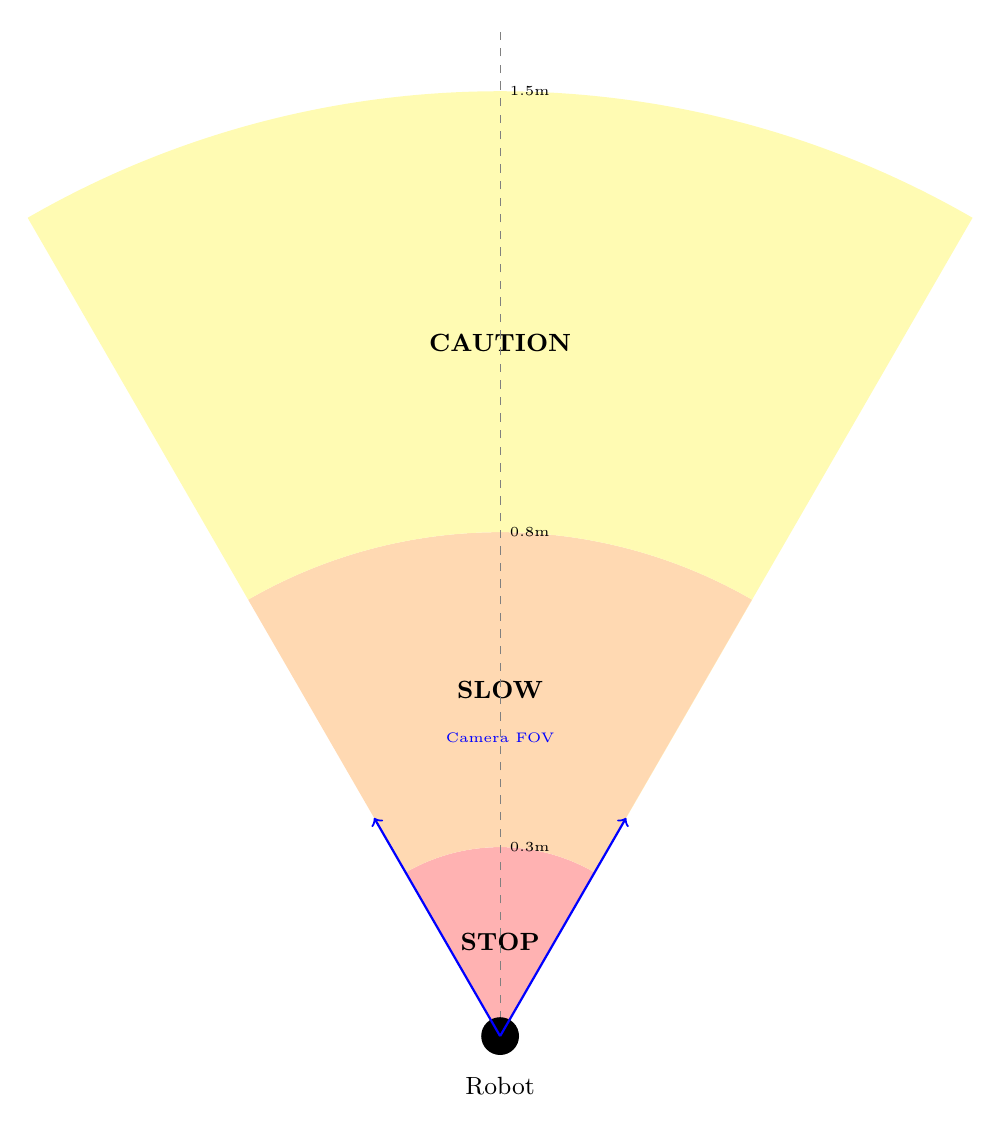
\begin{tikzpicture}[scale=0.8]
    % Draw safety zones as concentric arcs (robot FOV is forward-facing camera)
    \fill[red!30] (0,0) -- (60:3) arc (60:120:3) -- cycle;
    \fill[orange!30] (0,0) -- (60:8) arc (60:120:8) -- (120:3) arc (120:60:3) -- cycle;
    \fill[yellow!30] (0,0) -- (60:15) arc (60:120:15) -- (120:8) arc (120:60:8) -- cycle;

    % Labels for zones
    \node[font=\small\bfseries] at (90:1.5) {STOP};
    \node[font=\small\bfseries] at (90:5.5) {SLOW};
    \node[font=\small\bfseries] at (90:11) {CAUTION};

    % Distance markers
    \draw[dashed, gray] (0,0) -- (90:16);
    \node[right, font=\tiny] at (90:3) {0.3m};
    \node[right, font=\tiny] at (90:8) {0.8m};
    \node[right, font=\tiny] at (90:15) {1.5m};

    % Robot representation
    \fill[black] (0,0) circle (0.3);
    \node[below, font=\small] at (0,-0.5) {Robot};

    % Camera FOV indicator
    \draw[blue, thick, ->] (0,0) -- (60:4);
    \draw[blue, thick, ->] (0,0) -- (120:4);
    \node[blue, font=\tiny, above] at (90:4.5) {Camera FOV};

\end{tikzpicture}
\caption{Safety Zone Distances (Top-Down View)}
\end{figure}

\begin{table}[H]
\centering
\caption{Safety Zone Thresholds and Responses}
\begin{tabular}{|l|c|l|}
\hline
\textbf{Zone} & \textbf{Distance} & \textbf{Robot Response} \\
\hline
Emergency Stop (Red) & $<$ 0.3 m & Immediate stop, hold position \\
\hline
Slow Zone (Orange) & 0.3 -- 0.8 m & Reduce speed to 50\% of max \\
\hline
Caution Zone (Yellow) & 0.8 -- 1.5 m & Continue at current speed, log warning \\
\hline
Clear (Green) & $>$ 1.5 m & Normal operation \\
\hline
\end{tabular}
\end{table}

\subsection{Distance Estimation}

Since the USB camera provides 2D images without depth information, person distance is estimated using the detected bounding box height and a calibrated person height model:

\begin{lstlisting}[language=Python, caption=Distance estimation from bounding box]
# Calibration constants (adjust based on camera focal length and mounting)
FOCAL_LENGTH_PIXELS = 600  # Camera focal length in pixels
AVERAGE_PERSON_HEIGHT_M = 1.7  # Average adult height in meters
CAMERA_HEIGHT_M = 0.3  # Robot camera mounting height

def estimate_distance(bbox_height_pixels: int,
                      frame_height: int) -> float:
    """
    Estimate distance to person using pinhole camera model.

    distance = (real_height * focal_length) / image_height

    Args:
        bbox_height_pixels: Height of person bounding box in pixels
        frame_height: Total frame height in pixels

    Returns:
        Estimated distance in meters
    """
    if bbox_height_pixels <= 0:
        return float('inf')

    # Pinhole camera model
    distance = (AVERAGE_PERSON_HEIGHT_M * FOCAL_LENGTH_PIXELS) / bbox_height_pixels

    # Apply height correction (camera is not at ground level)
    # This is a simplification; more accurate models use full pose estimation
    distance = max(0.1, distance)

    return distance

# Calibration procedure:
# 1. Place person at known distance (e.g., 1.0m, 2.0m, 3.0m)
# 2. Record bounding box heights
# 3. Calculate FOCAL_LENGTH_PIXELS = (bbox_height * distance) / person_height
# 4. Average across multiple measurements
\end{lstlisting}

\subsection{Safety State Machine}

\begin{figure}[H]
\centering
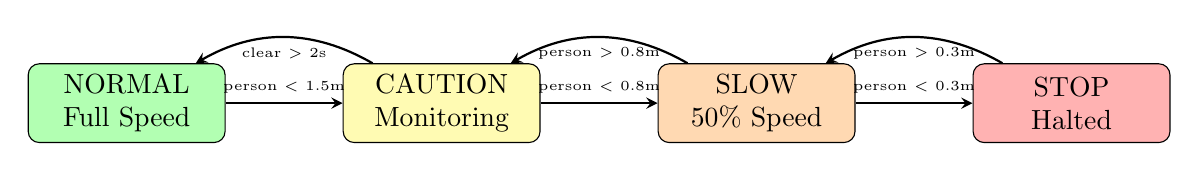
\begin{tikzpicture}[
    state/.style={draw, rectangle, rounded corners, minimum width=2.5cm, minimum height=1cm, align=center},
    arrow/.style={->, thick, >=stealth}
]
    % States
    \node[state, fill=green!30] (normal) at (0,0) {NORMAL\\Full Speed};
    \node[state, fill=yellow!30] (caution) at (4,0) {CAUTION\\Monitoring};
    \node[state, fill=orange!30] (slow) at (8,0) {SLOW\\50\% Speed};
    \node[state, fill=red!30] (stop) at (12,0) {STOP\\Halted};

    % Transitions
    \draw[arrow] (normal) -- node[above, font=\tiny] {person $<$ 1.5m} (caution);
    \draw[arrow] (caution) -- node[above, font=\tiny] {person $<$ 0.8m} (slow);
    \draw[arrow] (slow) -- node[above, font=\tiny] {person $<$ 0.3m} (stop);

    \draw[arrow, bend right=30] (caution) to node[below, font=\tiny] {clear $>$ 2s} (normal);
    \draw[arrow, bend right=30] (slow) to node[below, font=\tiny] {person $>$ 0.8m} (caution);
    \draw[arrow, bend right=30] (stop) to node[below, font=\tiny] {person $>$ 0.3m} (slow);

\end{tikzpicture}
\caption{CV Safety State Machine}
\end{figure}

\subsection{Integration with Navigation}

The CV safety system overrides navigation commands when necessary:

\begin{lstlisting}[language=Python, caption=SafetyController class]
from enum import Enum
from dataclasses import dataclass
from typing import Optional
import time

class SafetyState(Enum):
    NORMAL = "normal"
    CAUTION = "caution"
    SLOW = "slow"
    STOP = "stop"

@dataclass
class SafetyZones:
    EMERGENCY_STOP: float = 0.3   # meters
    SLOW_ZONE: float = 0.8        # meters
    CAUTION_ZONE: float = 1.5     # meters
    CLEAR_TIMEOUT: float = 2.0    # seconds before returning to normal

class SafetyController:
    def __init__(self):
        self.state = SafetyState.NORMAL
        self.last_detection_time: Optional[float] = None
        self.speed_multiplier = 1.0

    def update(self, person_distance: Optional[float]) -> SafetyState:
        """Update safety state based on nearest person distance."""
        current_time = time.time()

        if person_distance is None:
            # No person detected
            if self.last_detection_time is not None:
                elapsed = current_time - self.last_detection_time
                if elapsed > SafetyZones.CLEAR_TIMEOUT:
                    self._transition_to(SafetyState.NORMAL)
            return self.state

        self.last_detection_time = current_time

        # Determine appropriate state based on distance
        if person_distance < SafetyZones.EMERGENCY_STOP:
            self._transition_to(SafetyState.STOP)
        elif person_distance < SafetyZones.SLOW_ZONE:
            self._transition_to(SafetyState.SLOW)
        elif person_distance < SafetyZones.CAUTION_ZONE:
            self._transition_to(SafetyState.CAUTION)

        return self.state

    def _transition_to(self, new_state: SafetyState):
        if new_state != self.state:
            print(f"Safety state: {self.state.value} -> {new_state.value}")
            self.state = new_state
            self._update_speed_multiplier()

    def _update_speed_multiplier(self):
        multipliers = {
            SafetyState.NORMAL: 1.0,
            SafetyState.CAUTION: 1.0,
            SafetyState.SLOW: 0.5,
            SafetyState.STOP: 0.0,
        }
        self.speed_multiplier = multipliers[self.state]

    def apply_to_velocity(self, cmd_vel: tuple) -> tuple:
        """Apply safety multiplier to velocity command."""
        linear, angular = cmd_vel
        return (linear * self.speed_multiplier,
                angular * self.speed_multiplier)
\end{lstlisting}
